\documentclass{beamer}
\usepackage{tikz,amsmath,hyperref,graphicx,stackrel,animate,tipa}
\usetikzlibrary{positioning,shadows,arrows,shapes,calc}
\newcommand{\ipa}[1]{\textipa{#1}}
\newcommand{\argmax}{\operatornamewithlimits{argmax}}
\newcommand{\argmin}{\operatornamewithlimits{argmin}}
\mode<presentation>{\usetheme{Frankfurt}}
\DeclareMathOperator*{\softmax}{softmax}
\AtBeginSection[]
{
  \begin{frame}<beamer>
    \frametitle{Outline}
    \tableofcontents[currentsection,currentsubsection]
  \end{frame}
}
\title{Lecture 14: Log Viterbi and Scaled Forward-Backward}
\author{Mark Hasegawa-Johnson\\All content~\href{https://creativecommons.org/licenses/by-sa/4.0/}{CC-SA 4.0} unless otherwise specified.}
\date{ECE 417: Multimedia Signal Processing, Fall 2020}  
\begin{document}

% Title
\begin{frame}
  \maketitle
\end{frame}

% Title
\begin{frame}
  \tableofcontents
\end{frame}

%%%%%%%%%%%%%%%%%%%%%%%%%%%%%%%%%%%%%%%%%%%%
\section[Review]{Review: Hidden Markov Models}
\setcounter{subsection}{1}

\begin{frame}
  \frametitle{The Three Problems for an HMM}
  \begin{center}
    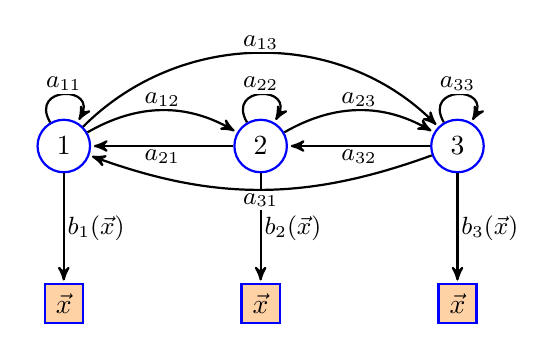
\begin{tikzpicture}[->,>=stealth',shorten >=1pt,auto,node distance=3cm,thick,
        state/.style={circle,thick,draw=blue,text=black,text centered,text width=0.25cm},
        obs/.style={rectangle,thick,draw=blue,text=black,fill=orange!35!white,text centered,text width=0.25cm}
      ]
      \node[state] (q1) at (0,0) {1};
      \node[state] (q2) at (2.5,0) {2};
      \node[state] (q3) at (5,0) {3};
      \node[obs] (x1) at (0,-2) {$\vec{x}$};
      \node[obs] (x2) at (2.5,-2) {$\vec{x}$};
      \node[obs] (x3) at (5,-2) {$\vec{x}$};
      \path[every node/.style={font=\sffamily\small,
  	  fill=white,inner sep=1pt}]
      (q1) edge [out=120,in=60,looseness=4] node {$a_{11}$} (q1)
      edge [out=30,in=150] node {$a_{12}$} (q2)
      edge [out=45,in=135] node {$a_{13}$} (q3)
      edge [out=-90,in=90] node {$b_1(\vec{x})$} (x1)
      (q2) edge [out=120,in=60,looseness=4] node {$a_{22}$} (q2)
      edge [out=180,in=0] node {$a_{21}$} (q1)
      edge [out=30,in=150] node {$a_{23}$} (q3)
      edge [out=-90,in=90] node {$b_2(\vec{x})$} (x2)
      (q3) edge [out=120,in=60,looseness=4] node {$a_{33}$} (q3)
      edge [out=180,in=0] node {$a_{32}$} (q2)
      edge [out=-160,in=-20] node {$a_{31}$} (q1)
      edge [out=-90,in=90] node {$b_3(\vec{x})$} (x3);
    \end{tikzpicture}
  \end{center}
  \begin{enumerate}
  \item {\bf Recognition:} Given two different HMMs, $\Lambda_1$ and
    $\Lambda_2$, and an observation sequence $X$.  Which HMM was more
    likely to have produced $X$?  In other words, 
    $p(X|\Lambda_1)>p(X|\Lambda_2)$?
  \item {\bf Segmentation:} What is $p(Q|X,\Lambda)$?
  \item {\bf Training:} Given an initial HMM $\Lambda$, and an
    observation sequence $X$, can we find $\Lambda'$ such that
    $p(X|\Lambda') > p(X|\Lambda)$?
  \end{enumerate}
\end{frame}

%%%%%%%%%%%%%%%%%%%%%%%%%%%%%%%%%%%%%%%%%%%%
\section[Recognition]{Recognition: The Scaled Forward Algorithm}
\setcounter{subsection}{1}

\begin{frame}
  \frametitle{The Forward Algorithm}

  Definition: $\alpha_t(i) \equiv p(\vec{x}_1,\ldots,\vec{x}_t,q_t=i|\Lambda)$.  Computation:
  \begin{enumerate}
  \item {\bf Initialize:}
    \[
    \alpha_1(i) = \pi_i b_i(\vec{x}_1),~~~1\le i\le N
    \]
  \item {\bf Iterate:}
    \begin{align*}
      \alpha_{t}(j) &= \sum_{i=1}^N \alpha_{t-1}(i) a_{ij}b_j(\vec{x}_t),~~1\le j\le N,~2\le t\le T
    \end{align*}
  \item {\bf Terminate:}
    \[
    p(X|\Lambda) = \sum_{i=1}^N \alpha_T(i)
    \]
  \end{enumerate}
\end{frame}


\begin{frame}
  \frametitle{Numerical Issues}

  The forward algorithm is susceptible to massive floating-point
  underflow problems. Consider this equation:
  \begin{align*}
    \alpha_{t}(j) &= \sum_{i=1}^N \alpha_{t-1}(i) a_{ij}b_j(\vec{x}_t)\\
    &= \sum_{q_1=1}^N\cdots\sum_{q_{t-1}=1}^N \pi_{q_1}b_{q_1}(\vec{x}_1)\cdots
    a_{q_{t-1}q_{t}}b_{q_t}(\vec{x}_t)
  \end{align*}
  First, suppose that $b_q(x)$ is discrete, with
  $k\in\left\{1,\ldots,K\right\}$.  Suppose $K\approx 1000$ and
  $T\approx 100$, in that case, each $\alpha_t(j)$ is:
  \begin{itemize}
  \item The sum of $N^T$ different terms, each of which is
  \item the product of $T$ factors, each of which is
  \item the product of two probabilities: $a_{ij}\sim\frac{1}{N}$ times
    $b_j(x)\sim\frac{1}{K}$, so
    \begin{displaymath}
      \alpha_T(j) \approx N^T\left(\frac{1}{NK}\right)^{T} \approx \frac{1}{K^T}\approx 10^{-300}
    \end{displaymath}
  \end{itemize}
\end{frame}

\begin{frame}
  \frametitle{Numerical Issues}

  Softmax observation probabilities are scaled similarly to discrete
  pmfs ($b_j(\vec{x})\sim\frac{1}{1000}$), but Gaussians are much
  worse. Suppose that $b_j(\vec{x})$ is Gaussian:
  \begin{displaymath}
    b_j(\vec{x})=
    \frac{1}{\prod_{d=1}^D\sqrt{2\pi\sigma_{jd}^2}}e^{-\frac{1}{2}\sum_{d=1}^D\frac{(x_d-\mu_{jd})^2}{\sigma_{jd}^2}}
  \end{displaymath}
  Suppose that $D\approx 30$.
  \begin{itemize}
  \item On average, $E\left[\frac{(x_d-\mu_{jd})^2}{\sigma_{jd}^2}\right]=1$,
  \item so  on average, $b_j(\vec{x})=\frac{1}{(2\pi)^{15}}e^{-15}=3\times 10^{-19}$.
  \end{itemize}
\end{frame}

\begin{frame}
  \frametitle{How to Solve Numerical Issues}

  \begin{itemize}
  \item Single-precision floating point can represent numbers as small
    as $2^{-127}$.
  \item One time step of the forward algorithm can be computed with no
    problem, but 100 time steps is impossible.
  \item Solution: re-normalize $\alpha_t(j)$ to $\hat\alpha_t(j)$
    after each time step, so that $\sum_j\hat\alpha_t(j)=1$.
  \end{itemize}
\end{frame}

\begin{frame}
  \frametitle{The Scaled Forward Algorithm}

  \begin{enumerate}
  \item {\bf Initialize:}
    \[
    \hat\alpha_1(i) = \frac{\pi_i b_i(\vec{x}_1)}{\sum_{\ell=1}^N\pi_\ell b_\ell(\vec{x}_1)}
    \]
  \item {\bf Iterate:}
    \begin{align*}
      \hat\alpha_{t}(j) &=
      \frac{\sum_{i=1}^N \hat\alpha_{t-1}(i) a_{ij}b_j(\vec{x}_t)}
      {\sum_{\ell=1}^N\sum_{i=1}^N \hat\alpha_{t-1}(i) a_{i\ell}b_\ell(\vec{x}_t)}
    \end{align*}
  \item {\bf Terminate:}
    \[
    p(X|\Lambda) = ????
    \]
  \end{enumerate}
\end{frame}

\begin{frame}
  \frametitle{What exactly is alpha-hat?}

  Let's look at this in more detail.  $\alpha_t(j)$ is defined to be
  $p(\vec{x}_1,\ldots,\vec{x}_t,q_t=j|\Lambda)$.  Let's define a
  ``scaling term,'' $G_t$, equal to the denominator in the scaled
  forward algorithm.  So, for example, at time $t=1$ we have:
  \begin{displaymath}
  G_1 = \sum_{\ell=1}^N \alpha_1(\ell)= \sum_{\ell=1}^N p(\vec{x}_1,q_1=\ell|\Lambda)
  = p(\vec{x}_1|\Lambda)
  \end{displaymath}
  and therefore
  \begin{displaymath}
  \hat\alpha_1(i) = \frac{\alpha_1(i)}{G_1} 
  = \frac{p(\vec{x}_1,q_1=i|\Lambda)}{p(\vec{x}_1|\Lambda)}
  = p(q_1=i|\vec{x}_1,\Lambda)
  \end{displaymath}
\end{frame}

\begin{frame}
  \frametitle{What exactly is alpha-hat?}
  At time $t$, we need a new intermediate variable.  Let's call it $\tilde\alpha_t(j)$:
  \begin{align*}
  \tilde\alpha_t(j) &= \sum_{i=1}^N \hat\alpha_{t-1}(i) a_{ij}b_j(\vec{x}_t)\\
  &= \sum_{i=1}^N p(q_{t-1}=i|\vec{x}_1,\ldots,\vec{x}_{t-1},\Lambda)p(q_t=j|q_{t-1}=i)p(\vec{x}_t|q_t=j)\\
  &= p(q_{t}=j,\vec{x}_t|\vec{x}_1,\ldots,\vec{x}_{t-1},\Lambda)\\
  G_t &= \sum_{\ell=1}^N \tilde\alpha_t(\ell) = p(\vec{x}_t|\vec{x}_1,\ldots,\vec{x}_{t-1},\Lambda)
  \end{align*}
  \begin{displaymath}
  \hat\alpha_t(j) = \frac{\tilde\alpha_t(j)}{G_t}
  = \frac{p(\vec{x}_t,q_t=j|\vec{x}_1,\ldots,\vec{x}_{t-1},\Lambda)}{p(\vec{x}_t|\vec{x}_1,\ldots,\vec{x}_{t-1},\Lambda)}
  = p(q_t=j|\vec{x}_1,\ldots,\vec{x}_t,\Lambda)
  \end{displaymath}
\end{frame}

\begin{frame}
  \frametitle{Scaled Forward Algorithm: The Variables}

  So we have not just one, but two new variables:
  \begin{enumerate}
  \item The scaled forward probability:
    \begin{displaymath}
      \hat\alpha_t(j) = p(q_t=j|\vec{x}_1,\ldots,\vec{x}_{t},\Lambda)
    \end{displaymath}
  \item The scaling factor:
    \begin{displaymath}
      G_t = p(\vec{x}_t|\vec{x}_1,\ldots,\vec{x}_{t-1},\Lambda)
    \end{displaymath}
  \end{enumerate}
\end{frame}

\begin{frame}
  \frametitle{The Solution}

  The second of those variables is interesting because we want $p(X|\Lambda)$, which
  we can now get from the $G_t$s---we no longer actually need the $\alpha$s for this!
  \begin{displaymath}
    p(X|\Lambda) = p(\vec{x}_1|\Lambda )p(\vec{x}_2|\vec{x}_1,\Lambda)p(\vec{x}_3|\vec{x}_1,\vec{x}_2,\Lambda )\cdots= \prod_{t=1}^T G_t
  \end{displaymath}
  But that's still not useful, because if each $G_t\sim 10^{-19}$,
  then multiplying them all together will result in floating point
  underflow.  So instead, it is better to compute
  \begin{align*}
    \ln p(X|\Lambda) = \sum_{t=1}^T \ln G_t
  \end{align*}
\end{frame}

\begin{frame}
  \frametitle{The Scaled Forward Algorithm}

  \begin{enumerate}
  \item {\bf Initialize:}
    \[
    \hat\alpha_1(i) = \frac{1}{G_1}\pi_i b_i(\vec{x}_1)
    \]
  \item {\bf Iterate:}
    \begin{align*}
      \hat\alpha_{t}(j) &=
      \frac{1}{G_t}\sum_{i=1}^N \hat\alpha_{t-1}(i) a_{ij}b_j(\vec{x}_t)
    \end{align*}
  \item {\bf Terminate:}
    \[
    \ln p(X|\Lambda) = \sum_{t=1}^T \ln G_t
    \]
  \end{enumerate}
\end{frame}

%%%%%%%%%%%%%%%%%%%%%%%%%%%%%%%%%%%%%%%%%%%%
\section[Segmentation]{Segmentation: The Viterbi Algorithm}
\setcounter{subsection}{1}

\begin{frame}
  \frametitle{What About State Sequences?}

  \begin{itemize}
  \item Remember when we first derived $\gamma_t(i)$, I pointed out a
    problem: $\gamma_t(i)$ only tells us about one frame at a time!
    It doesn't tell us anything about the probability of a sequence of
    states, covering a sequence of frames.
  \item Today, let's find a complete solution.  Let's find the most
    likely state sequence covering the entire utterance:
    \[
    Q^*  = \argmax_Q p(Q,X|\Lambda)
    \]
  \end{itemize}
\end{frame}

\begin{frame}
  \frametitle{The Max-Probability State Sequence}

  The problem of finding the max-probability state sequence is just as
  hard as the problem of finding $p(X|\Lambda)$, for exactly the same
  reason:
  \begin{align*}
    \max_Q p(Q,X|\Lambda) &= \max_{q_T=1}^N\cdots\max_{q_1=1}^N p(Q,X|\Lambda)
  \end{align*}
  which has complexity ${\mathcal O}\left\{N^T\right\}$.
\end{frame}
\begin{frame}
  \frametitle{The Viterbi Algorithm}
  
  Remember that we solved the recognition probability using a
  divide-and-conquer kind of dynamic programming algorithm, with the
  intermediate variable
  \begin{align*}
  \alpha_t(j) &\equiv p(\vec{x}_1,\ldots,\vec{x}_t,q_t=j|\Lambda)\\
  &=\sum_{q_{t-1}}\cdots\sum_{q_1}
  p(\vec{x}_1,\ldots,\vec{x}_t,q_1,\ldots,q_{t-1},q_t=j|\Lambda)
  \end{align*}
  The segmentation problem is solved using a similar dynamic
  programming algorithm called the Viterbi algorithm, with a slightly
  different intermediate variable:
  \[
  \delta_t(j)\equiv \max_{q_{t-1}}\cdots\max_{q_1}
  p(\vec{x}_1,\ldots,\vec{x}_t,q_1,\ldots,q_{t-1},q_t=j|\Lambda)
  \]
\end{frame}

\begin{frame}
  \frametitle{The Viterbi Algorithm}
  Keeping in mind the definition
  $\delta_t(j)\equiv\max_{q_{t-1}}\cdots\max_{q_1}p(\vec{x}_1,\ldots,\vec{x}_t,q_1,\ldots,q_{t-1},q_t=j|\Lambda)$,
  we can devise an efficient algorithm to compute it:
  \begin{enumerate}
  \item {\bf Initialize:}
    \[
    \delta_1(i) = \pi_i b_i(\vec{x}_1)
    \]
  \item {\bf Iterate:}
    \begin{align*}
      \delta_{t}(j) &= \max_{i=1}^N \delta_{t-1}(i) a_{ij}b_j(\vec{x}_t)
    \end{align*}
  \item {\bf Terminate:}
    The maximum-probability final state is $q_T^* = \argmax_{j=1}^N \delta_T(j)$.  But what
    are the best states at all of the previous time steps?
  \end{enumerate}
\end{frame}

\begin{frame}
  \frametitle{Backtracing}

  We can find the optimum states at all times, $q_t^*$, by keeping a
  {\bf backpointer} $\psi_t(j)$ from every time step.  The backpointer
  points to the state at time $t-1$ that is most likely to have
  preceded state $j$ at time $t$:
  \begin{align*}
    \psi_{t}(j) &= \argmax_i\cdots\max_{q_1}p(\vec{x}_1,\ldots,\vec{x}_t,q_1,\ldots,q_{t-1}=i,q_t=j|\Lambda)\\
    &= \argmax_{i=1}^N \delta_{t-1}(i) a_{ij}b_j(\vec{x}_t)
  \end{align*}
\end{frame}

\begin{frame}
  \frametitle{Backtracing}

  If we have the backpointers available, then we can get the entire
  maximum-probability state sequence by {\bf backtracing} after we
  terminate:
  \begin{itemize}
  \item {\bf Terminate:} Once we get to time $t=T$, we choose the most
    probable final state.
    \begin{itemize}
    \item If we already know which state we want to end in, then we
      just choose that state as $q_T^*$.
    \item If we don't already know, then we choose
      $q_T^*=\argmax_{j}\delta_T(j)$
    \end{itemize}
  \item {\bf Backtrace:} Having found the final state, we work
    backward, by way of the {\bf backpointers}, $\psi_t(j)$:
    \begin{align*}
      q_t^* &= \psi_{t+1}\left(q_{t+1}^*\right),~~~T-1\ge t\ge 1
    \end{align*}
  \end{itemize}
\end{frame}

\begin{frame}
  \frametitle{The Viterbi Algorithm}
  \begin{enumerate}
  \item {\bf Initialize:}
    \[
    \delta_1(i) = \pi_i b_i(\vec{x}_1)
    \]
  \item {\bf Iterate:}
    \begin{align*}
      \delta_{t}(j) &= \max_{i=1}^N \delta_{t-1}(i) a_{ij}b_j(\vec{x}_t)\\
      \psi_{t}(j) &= \argmax_{i=1}^N \delta_{t-1}(i) a_{ij}b_j(\vec{x}_t)
    \end{align*}
  \item {\bf Terminate:}
    \begin{align*}
      q_T^* &= \argmax_{j=1}^N \delta_T(j)
    \end{align*}
  \item {\bf Backtrace:}
    \begin{align*}
      q_t^* &= \psi_{t+1}\left(q_{t+1}^*\right)
    \end{align*}
  \end{enumerate}
\end{frame}

\begin{frame}
  \frametitle{Example}
  \centerline{\includegraphics[height=2.5in]{exp/An_example_of_HMM.png}}
  \begin{tiny}
    An example of HMM, GFDL by Reelsun, 2012,
    \url{https://commons.wikimedia.org/wiki/File:An_example_of_HMM.png}
  \end{tiny}
\end{frame}

\begin{frame}
  \frametitle{Example}
  \centerline{\animategraphics[loop,controls,width=4.5in]{1}{exp/Viterbi_animated_demo-}{0}{4}}
  \begin{tiny}
    Viterbi animated demo, GFDL by Reelsun, 2012,
    \url{https://commons.wikimedia.org/wiki/File:Viterbi_animated_demo.gif}
  \end{tiny}
\end{frame}

\begin{frame}
  \frametitle{Numerical Problems}

  Viterbi algorithm has the same floating-point underflow problems as
  the Forward algorithm.  But this time, there is an easy solution,
  because the log of the max is equal to the max of the log:
  \begin{align*}
    \ln\delta_{t}(j) &= \ln\left(\max_{i=1}^N \delta_{t-1}(i) a_{ij}b_j(\vec{x}_t)\right)\\
    &= \max_{i=1}^N\left(\ln\delta_{t-1}(i)+ \ln a_{ij}+ \ln b_j(\vec{x}_t)\right)
  \end{align*}
\end{frame}
      
\begin{frame}
  \frametitle{The Log-Viterbi Algorithm}

  \begin{enumerate}
  \item {\bf Initialize:}
    \[
    \ln\delta_1(i) = \ln\pi_i +\ln b_i(\vec{x}_1)
    \]
  \item {\bf Iterate:}
    \begin{align*}
      \ln\delta_{t}(j) &= \max_{i=1}^N \left(\ln\delta_{t-1}(i) +\ln a_{ij}+ \ln b_j(\vec{x}_t)\right)\\
      \psi_{t}(j) &= \argmax_{i=1}^N \left(\ln\delta_{t-1}(i) +\ln a_{ij}+ \ln b_j(\vec{x}_t)\right)
    \end{align*}
  \item {\bf Terminate:}
    Choose the known final state $q_T^*$.
  \item {\bf Backtrace:}
    \begin{align*}
      q_t^* &= \psi_{t+1}\left(q_{t+1}^*\right)
    \end{align*}
  \end{enumerate}
\end{frame}

%%%%%%%%%%%%%%%%%%%%%%%%%%%%%%%%%%%%%%%%%%%%
\section[Training]{Training: The Scaled Backward Algorithm}
\setcounter{subsection}{1}

\begin{frame}
  \frametitle{Baum-Welch Re-estimation}

  Unfortunately, the Viterbi algorithm doesn't solve the problem of
  training.  We still need:
  \begin{align*}
    \xi_t(i,j) &\equiv p(q_t=i,q_{t+1}=j|X,\Lambda)\\
    &= \frac{\alpha_t(i)a_{ij}b_j(\vec{x}_{t+1})\beta_{t+1}(j)}
       {\sum_{k=1}^N\sum_{\ell=1}^N \alpha_t(k)a_{k\ell}b_\ell(\vec{x}_{t+1})\beta_{t+1}(\ell)}
  \end{align*}
  We have a numerically-safe algorithm for finding $\hat\alpha_t(j)$.
  Can we use that, somehow?
\end{frame}

\begin{frame}
  \frametitle{Scaled Baum-Welch Re-estimation}

  \begin{itemize}
  \item We already have
    \begin{displaymath}
      \hat\alpha_t(i) = \frac{\alpha_t(i)}{\prod_{\tau=1}^{t} G_\tau} 
    \end{displaymath}
  \item Suppose we also define
    \begin{displaymath}
      \hat\beta_{t+1}(j) = \frac{\beta_{t+1}(j)}{\prod_{\tau=(t+1)}^T G_\tau}
    \end{displaymath}
  \item Then we get
    \begin{align*}
      &\frac{\hat\alpha_t(i)a_{ij}b_j(\vec{x}_{t+1})\hat\beta_{t+1}(j)}{\sum_{k=1}^N\sum_{\ell=1}^N \hat\alpha_t(k)a_{k\ell}b_\ell(\vec{x}_{t+1})\hat\beta_{t+1}(\ell)}\\
      &= \frac{\frac{1}{\prod_{\tau=1}^TG_\tau}\alpha_t(i)a_{ij}b_j(\vec{x}_{t+1})\beta_{t+1}(j)}{\frac{1}{\prod_{\tau=1}^TG_\tau}\sum_{k=1}^N\sum_{\ell=1}^N\alpha_t(k)a_{k\ell}b_\ell(\vec{x}_{t+1})\beta_{t+1}(\ell)}\\
      &= \xi_t(i,j)
    \end{align*}
  \end{itemize}
\end{frame}
  
\begin{frame}
  \frametitle{The Scaled Backward Algorithm}

  \begin{enumerate}
  \item {\bf Initialize:}
    \[
    \hat\beta_T(i) = 1,~~1\le i\le N
    \]
  \item {\bf Iterate:}
    \begin{align*}
      \hat\beta_{t}(i) &= \frac{1}{G_t}\sum_{j=1}^N a_{ij}b_j(\vec{x}_{t+1})\hat\beta_{t+1}(j)
    \end{align*}
  \end{enumerate}
  The scaling constant, $G_t$, can be the same for forward algorithm,
  but doesn't have to be.  I get better results using other
  normalizing constants, for example, $\sum_i\hat\beta_t(i)=1$ for
  $t<T$.
\end{frame}

%%%%%%%%%%%%%%%%%%%%%%%%%%%%%%%%%%%%%%%%%%%%
\section[Summary]{Summary}
\setcounter{subsection}{1}

\begin{frame}
  \frametitle{The Scaled Forward Algorithm}

  \begin{enumerate}
  \item {\bf Initialize:}
    \[
    \hat\alpha_1(i) = \frac{1}{G_1}\pi_i b_i(\vec{x}_1)
    \]
  \item {\bf Iterate:}
    \begin{align*}
      \hat\alpha_{t}(j) &=
      \frac{1}{G_t}\sum_{i=1}^N \hat\alpha_{t-1}(i) a_{ij}b_j(\vec{x}_t)
    \end{align*}
  \item {\bf Terminate:}
    \[
    \ln p(X|\Lambda) = \sum_{t=1}^T \ln G_t
    \]
  \end{enumerate}
\end{frame}

\begin{frame}
  \frametitle{The Log-Viterbi Algorithm}

  \begin{enumerate}
  \item {\bf Initialize:}
    \[
    \ln\delta_1(i) = \ln\pi_i +\ln b_i(\vec{x}_1)
    \]
  \item {\bf Iterate:}
    \begin{align*}
      \ln\delta_{t}(j) &= \max_{i=1}^N\left(\ln\delta_{t-1}(i) +\ln a_{ij}+ \ln b_j(\vec{x}_t)\right)\\
      \psi_{t}(j) &= \argmax_{i=1}^N\left(\ln\delta_{t-1}(i) +\ln a_{ij}+ \ln b_j(\vec{x}_t)\right)
    \end{align*}
  \item {\bf Terminate:}
    Choose the known final state $q_T^*$.
  \item {\bf Backtrace:}
    \begin{align*}
      q_t^* &= \psi_{t+1}\left(q_{t+1}^*\right)
    \end{align*}
  \end{enumerate}
\end{frame}

\begin{frame}
  \frametitle{Scaled Baum-Welch Re-estimation}

  \begin{align*}
    \xi_t(i,j) &\equiv p(q_t=i,q_{t+1}=j|X,\Lambda)\\
    &= \frac{\hat\alpha_t(i)a_{ij}b_j(\vec{x}_{t+1})\hat\beta_{t+1}(j)}
       {\sum_{k=1}^N\sum_{\ell=1}^N \hat\alpha_t(k)a_{k\ell}b_\ell(\vec{x}_{t+1})\hat\beta_{t+1}(\ell)}
  \end{align*}
\end{frame}

\end{document}

